\section{Process Analysis}
Process analysis aims to evaluate the performance and efficiency of business processes, to guide process improvement initiatives.
Taking as input a \textit{as-is} process model, it provides insights on weaknesses and their impact.
We can distinguish between two main types of analysis:
\begin{itemize}
    \item \textbf{Qualitative Analysis}: focuses on identifying inefficiencies, bottlenecks, and areas for improvement within a process.
    \item \textbf{Quantitative Analysis}: focuses on measuring and evaluating the performance of a process using various metrics.
\end{itemize}

\subsection{Process Qualitative Analysis}
\subsubsection{Value-added analysis}
This kind of analysis focuses on \textbf{identifying and categorizing} activities within a business process based on their contribution to the overall value delivered to customers or stakeholders.
After that we can optimize the process by \textbf{eliminating} non-value-adding activities.
\paragraph{Identification} We break down the process into atomic steps, 
examining each one of them to determine its category among the following:
\begin{itemize}
    \item \textbf{Value-added activities}: directly contribute to delivering value or satisfaction to the customer
        \begin{itemize}
            \item Is the customer willing to pay for this activity?
            \item Would the customer agree that this step is necessary to achieve their goals?
            \item If the step were eliminated, would the customer notice a difference in the final product or service?
        \end{itemize}
    \item \textbf{Business value-added activities}: necessary for the business operation but do not directly add value from the customer's perspective
        \begin{itemize}
            \item Is this step required in order to collect revenue, to improve or grow the business?
            \item Would the business potentially suffer if this step were eliminated?
            \item Does it reduce risk of business losses?
            \item Is this step required to comply with regulations or legal requirements?
        \end{itemize}
    \item \textbf{Non-value-adding activities}: do not add value and are not necessary for the business (everything that is not VA or BVA).
    This usually includes handovers, delays, rework, etc.
\end{itemize}

\paragraph{Waste Elimination} After identifying and categorizing the activities, we can remove NVA activities and 
carefully evaluate BVA activities to see if they can be optimized or eliminated without negatively impacting the business.
We have different sources of waste:
\begin{itemize}
    \item \textbf{Move}:
        \begin{itemize}
            \item \textbf{Transportation}: send or receive materials or document taken as input or output of an activity;
            \item \textbf{Motion}: movement of resources (people, materials) internally within the process.
        \end{itemize}
    \item \textbf{Hold}:
        \begin{itemize}
            \item \textbf{Inventory}: accumulation of materials or documents waiting to be processed (Work in Progress - WIP);
            \item \textbf{Waiting}: task waiting for input data or resource availability, or resources waiting for task assignment.
        \end{itemize}
    \item \textbf{Over-do}:
        \begin{itemize}
            \item \textbf{Defects}: correcting or compensating for errors or mistakes in the process (rework loops);
            \item \textbf{Over-processing}: tasks performed unnecessarily given the outcome required by the customer;
            \item \textbf{Over-production}: unnecessary process instances are performed, producing outcomes that do not add value upon the completion of the process.
        \end{itemize}
\end{itemize}

\subsection{Process Quantitative Analysis}
The process performance can be measured through different dimensions:
\begin{itemize}
    \item \textbf{Time}: how long it takes to complete a process or specific activities within the process;
    \item \textbf{Cost}: the expenses incurred to execute the process, including labor, materials, and overhead costs;
    \item \textbf{Quality}: the degree to which the process meets customer requirements and expectations.
\end{itemize}

\subsubsection{Time Measures}

\paragraph{Cycle (throughput) time}: the time between start and completion of a process instance.
It can be measured as:
\begin{equation}
    \text{Cycle throughput time} = \text{Processing Time (PT)} + \text{Waiting Time (WT)}
\end{equation}
where:
\begin{itemize}
    \item \textbf{Processing Time (PT)}: time taken by value-adding activities
    \item  \textbf{Waiting Time (WT)}: time spent in non-value-adding activities
\end{itemize}

The result can be different from a simply sum, depending on the process structure (e.g., parallel paths, loops, etc.).
\begin{figure}[H]
    \label{fig:cycle_time_table}
    \centering
    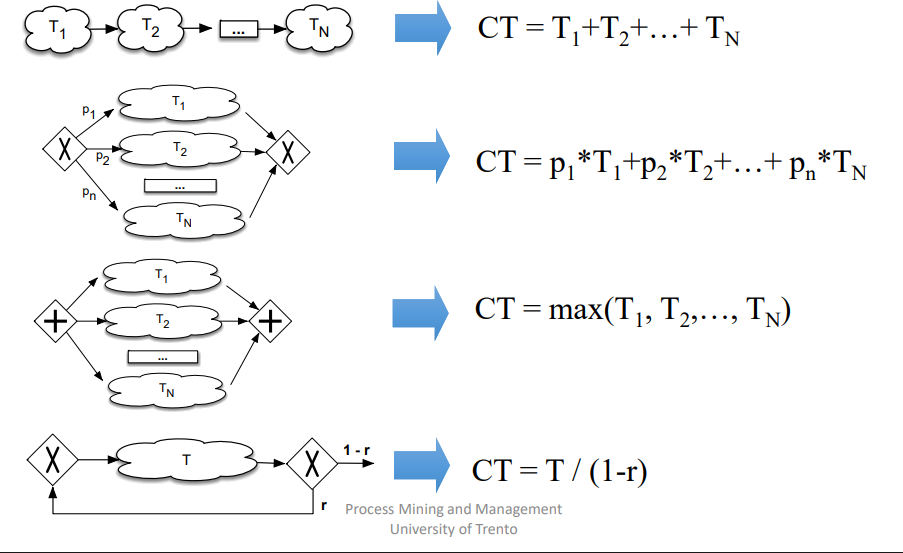
\includegraphics[width=0.9\textwidth]{../images/chapters/bpmn_analysis/CTE_table.png}
    \caption{Cycle Time Calculation Table}
\end{figure}
\begin{itemize}
    \item In case of \textbf{sequential} activities, the cycle time is the sum of the cycle times of each activity;
    \item In case of \textbf{exclusive choices} (XOR), the cycle time is the weighted average of the cycle times of each branch, using the branching probabilities as weights;
    \item In case of \textbf{parallel} activities, the cycle time is the maximum cycle time among the parallel branches;
    \item In case of \textbf{loops}, the cycle time is the sum of the cycle time of the activities inside the loop, divided by the probability of exiting the loop.
\end{itemize}

\paragraph{Cycle Time Efficiency}
Given the cycle time, we can calculate the efficiency of the process.
The Cycle Time Efficiency (CTE) is a measure of how efficiently a process is executed, focusing on the proportion of time spent on value-adding activities compared to the total cycle time.
It is calculated as:
\begin{equation}
    \text{CTE} = \frac{\text{Processing Time (PT)}}{\text{Cycle throughput time}} 
\end{equation}

\subsubsection{Cost Measures}
\paragraph{Per-instance Cost}
The per-instance cost of a process measures the total cost incurred to complete a single instance of the process.
It is calculated as:
\begin{equation}
    \text{Per-instance Cost} = \text{Processing cost} + \text{Cost of waste}
\end{equation}
where:
\begin{itemize}
    \item \textbf{Processing cost}: cost associated with value-adding activities
    \item  \textbf{Cost of waste}: cost associated with non-value-adding activities
\end{itemize}

\subsubsection{Work-In-Progress (WIP)}
Work-In-Progress (WIP) refers to the number of process instances that are currently being executed but have not yet been completed.
WIP is a form of waste. 
Using Little's Law, we can relate WIP to the arrival rate and cycle time:
\begin{equation}
    \text{WIP} = \lambda \times \text{Cycle Time}
\end{equation}
where $\lambda$ is the arrival rate (number of cases arriving per time unit).
Its limitation is that we can't estimate waiting times or queue lengths.